\section{Detection Strategies}
\label{sec:background:detection_strategies}

Text extraction strategies have seen continuing interest in the literature, with many comprehensive surveys assessing the state of the art \cite{Chen:2000ua, Jung:2004uwa, Zhang:2008vfa, Liang:2005uy, Jung:2004uw}. It is widely demonstrated that if text within an unstructured scene is \textit{detected} reliably, then existing \gls{ocr} engines can suitably extract these characters \citep{Smith:2007dc} once they exist in a structured context; thus not every extraction pipeline needs to self-contain a recognition strategy if commercial \gls{ocr} packages suffice. A survey into the two prominent detection strategies are given in \cref{sec:detection:cc,sec:detection:learning}.

These two prominent strategies have a varied nomenclature: (1) the \gls{cc}-based (or \textit{region}-based) approach, that utilise different region properties (e.g., colour, edges, \glspl{cc}) \citep{Jain:1998wd, Kim:1996tw, Liu:2006wh, Chen:2011ul, Li:2012wd, Zhang:2011cl, Shivakumara:2011dn, Epshtein:2010tj, Zhang:2010wa, Shivakumara:2010wu, Liu:2008tz, Subramanian:2007tf, Lee:2010vv, Sun:2010tg} for unsupervised extraction; and, (2) learning-based (or \textit{texture}-based) approach, which uses unique texture properties to supervise extraction text from its background \citep{Ye:2005wu,XiangrongChen:2004ha,Pan:2010cj,Gllavata:2004vq,Minetto:2010tg,Phan:2009bc,Lee:2003cn,Lienhart:2002ub,Li:2000uf,Wang:2009il,Dalal:2005jq,Hanif:2009tm,Tu:2003tg,Chen:2005wv}. Some authors have proposed methods that mix both supervised and unsupervised techniques \citep{Mutch:2006ub, Mairal:2008uw, Bengio:2006vb}.

\subsection{Connected Component-based techniques}
\label{sec:detection:cc}

\glsx{cc}-based approaches generate separated \glspl{cc} using properties such as stroke width, pixel colour and edges, typically applying geometric and texture filters to reduce false positives. Neighbouring pixels are then `grouped' using an algorithm such as the one originally presented by \citet{Horn:1986vc}. 

Previous work required the use of a scanning window \citep{XiangrongChen:2004ha, Lienhart:2002ub, Jung:2009do} that is limited by a constant image scale and discrete orientations of the sliding (thereby preventing text strokes in non-linear directions). \citet{Subramanian:2007tf} overcame this limitation by implementing an algorithm to detect text strokes by scanning an image horizontally and looking for sudden changes in background intensity (\cref{fig:background:detection:cc:subramanian2007_intensity}b). However, this algorithm assumes a darker text on a lighter background to find such intensity changes, and consequently there are numerous parameters that must be fine-tuned. Additionally, the algorithm is only able to detect horizontal text only, and detected strokes are not grouped into characters, words and sentences.

\begin{figure}[h]
  \centering
  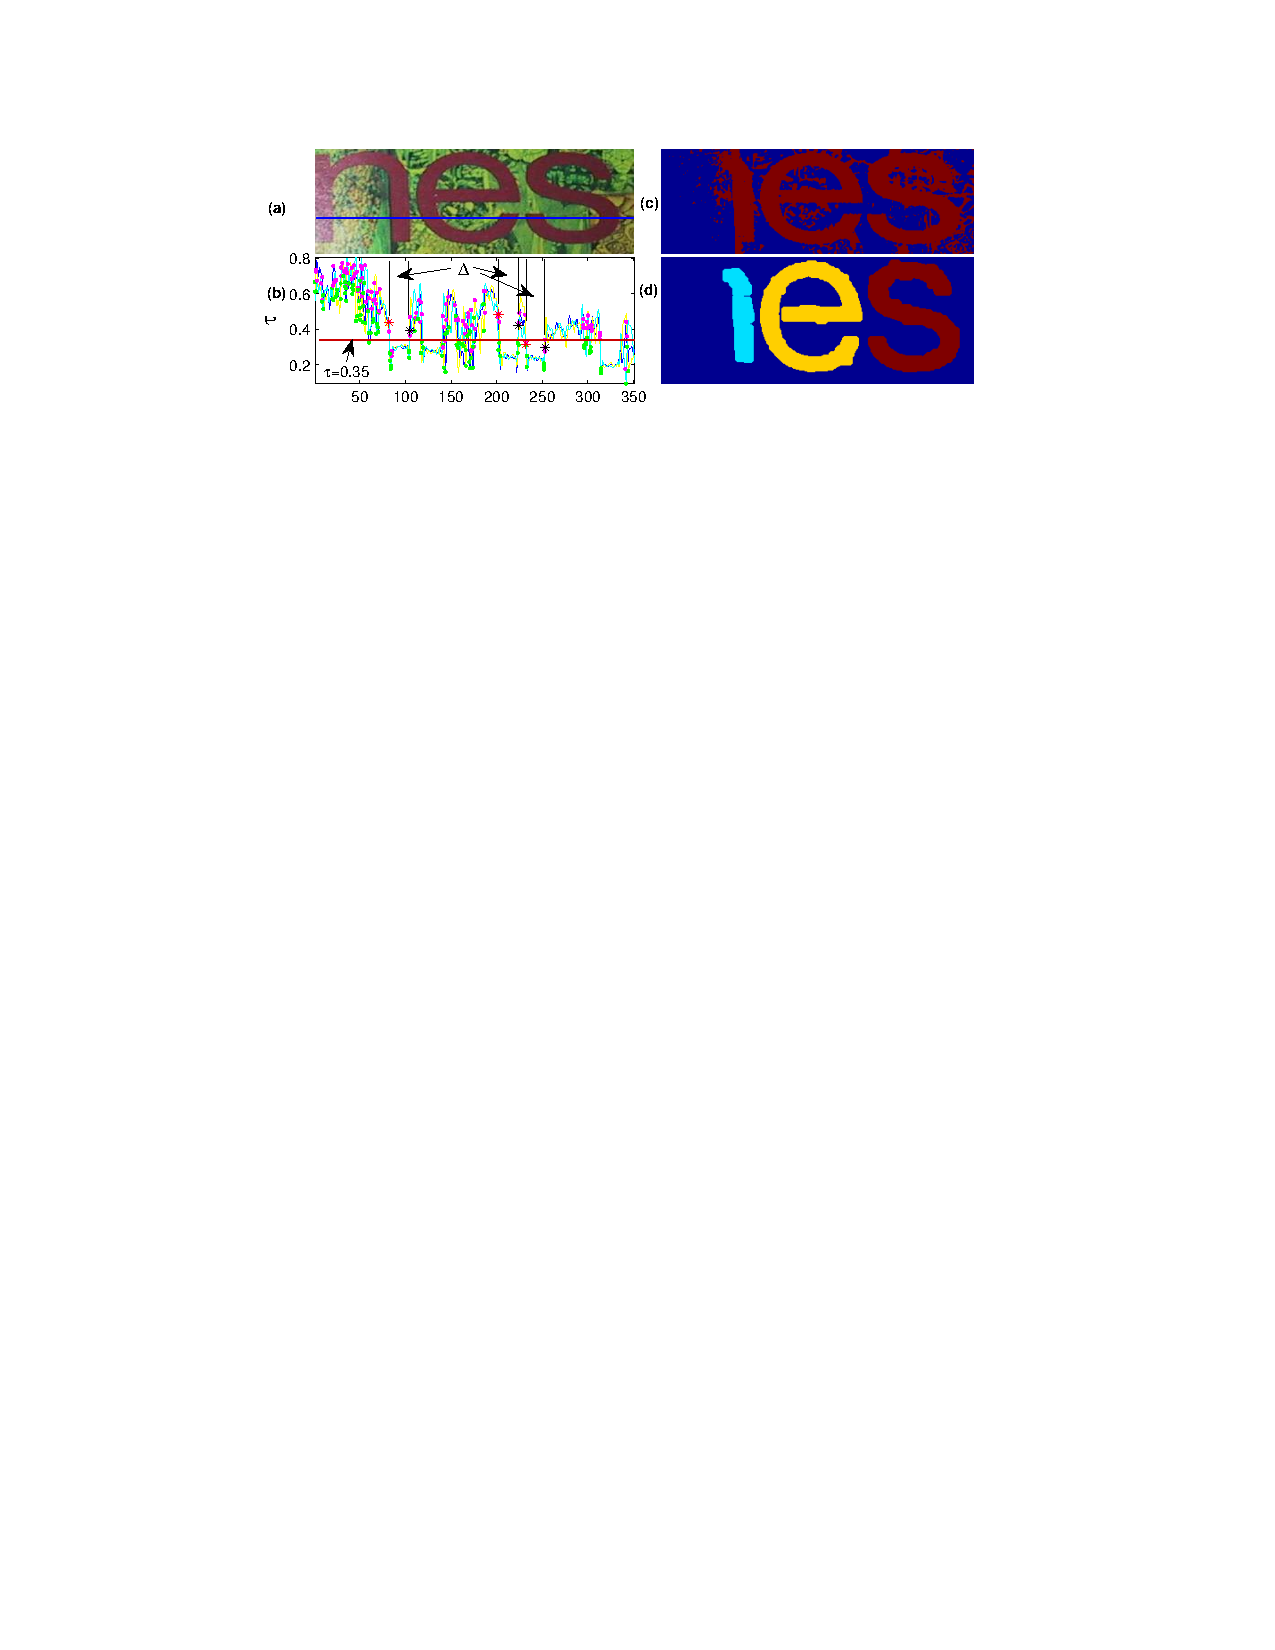
\includegraphics[width=0.8\textwidth]{images/background/subramanian2007_intensity}
  \caption[Stroke analysis from \citet{Subramanian:2007tf}]{A study from \citet{Subramanian:2007tf} showed that stroke width could be determined from (a) the original image; (b) intensity plots of the image to determine stroke regions ($\tau$ is the intensity threshold and $\Delta$ is the stroke width); (c) the intensity at an optimal threshold; (d) the final thresholded image after morphological operations and \gls{cc} analysis.}
  \label{fig:background:detection:cc:subramanian2007_intensity}
\end{figure}

A study by \citet{Epshtein:2010tj} (and coincidentally \citet{Zhang:2011cl}) built on the idea presented by \citeauthor{Subramanian:2007tf}, and introduced the concept of \gls{swt}, a local image operator that determines the most likely stroke of a given pixel by computing the per-pixel width. This was later expanded in \citet{Srivastav:2008ge}. The \gls{swt} approach overcame previous limitations by introducing a system that can detect text regardless of size, typeface, direction and language, making it one of the first widely cited multilingual text detection algorithms. Additionally, \gls{swt} overcame methods that required the use of an OCR filtering stage to reduce false positives \citep{Chen:2004tx, XiangrongChen:2004ha, Ye:2005wu}. A sample of \gls{swt} is shown in \cref{fig:background:detection:cc:epshtein2010_swt}.

\begin{figure}[h]
  \centering
  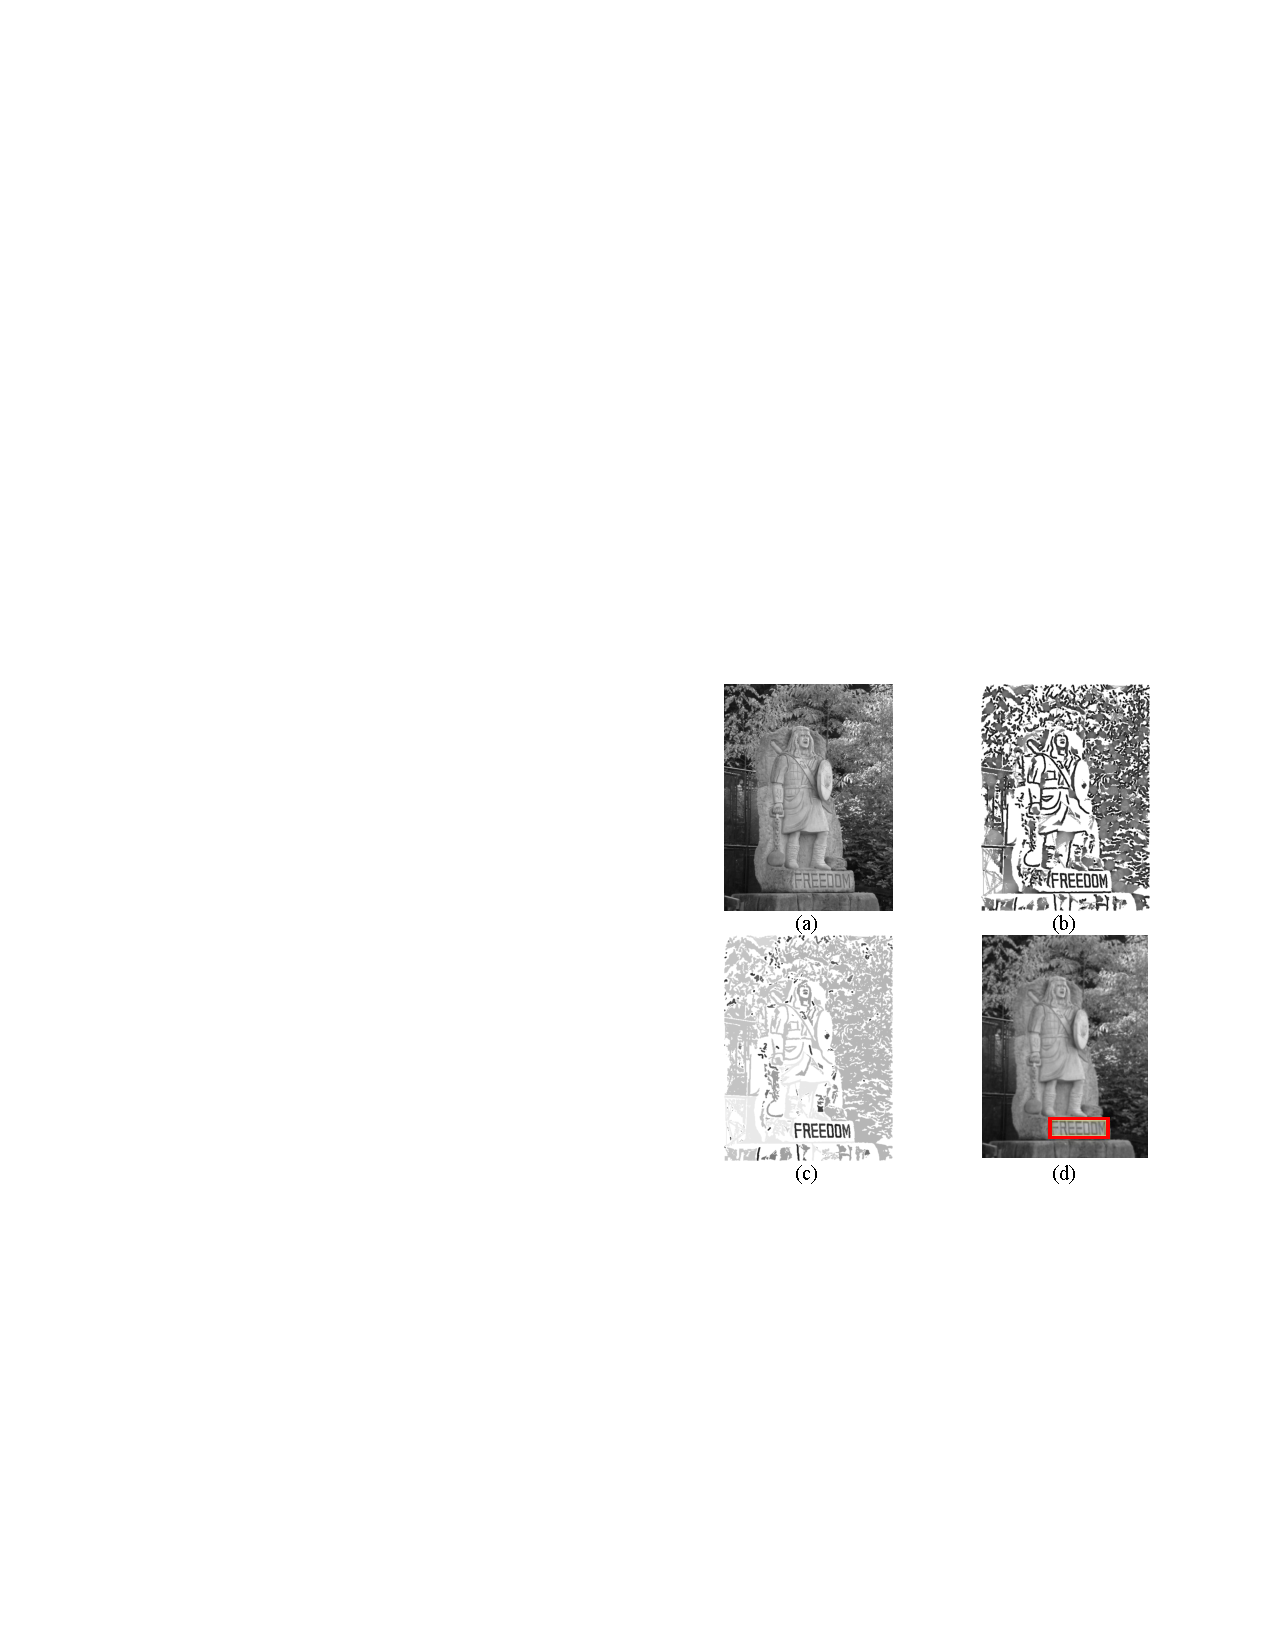
\includegraphics[width=0.5\textwidth]{images/background/epshtein2010_swt}
  \caption[Stroke Width Transformation from \citet{Epshtein:2010tj}]{The \glsx{swt} approach introduced in \citep{Epshtein:2010tj}. The original image (a) is converted to a binarised array with the most likely stroke width per-pixel (b), piping the information into geometric filtering (c) as text maintains fixed stroke width (excluding false positives such as foliage). The resulting detected text is shown in (d).}
  \label{fig:background:detection:cc:epshtein2010_swt}
\end{figure}

It is common to see edges computed from a raw image using the Canny-Edge Detection algorithm \citep{Canny:1986uw}. This was successfully applied in various \gls{cc}-based studies \citep{Epshtein:2010tj, Chen:2011ul, Zhang:2010wa}. While different researchers have exploited \gls{swt} and adapted it further \cite{Shivakumara:2011dn, Zhang:2011cl}, when opposite edges are not parallel, the \gls{swt} forms candidates with holes appearing in stroke curves or joints. This is due to candidates formed by shooting rays from detected the edges along the gradient found, removing the rays if terminated by another edge pixel of a perpendicular gradient. Further limitations include undetected stronger highlights, blurry text, and text with a wide curvature.

An alternate approach that overcomes this limitation was introduced by \citet{Chen:2011ul}, where the complimentary properties of Canny-Edges \citep{Canny:1986uw} and \glspl{mser} \citep{Matas:2002tp} were combined. \gls{mser} is a detection mechanism suited for region-based detection, is robust against varying viewpoints, scales and illuminations \citep{Mikolajczyk:2005tb}, and can be extracted from images efficiently \citep{Nister:2008vk}. A limitation of \gls{mser} is its sensitivity to image blur \citep{Mikolajczyk:2005tb}, but \citeauthor{Chen:2011ul} demonstrated that \gls{mser} can be edge-enhanced using Canny-Edges on a contrast-enhanced image (\cref{fig:background:detection:cc:chen2011_mser}), achieving comparable results to \gls{swt} presented by \citet{Epshtein:2010tj}. Multiple works have utilised \glspl{mser} in a wide range of applications, such as their use in teaching \glspl{cnn} and real-time text extraction \cite{Li:2012wd,Gonzalez:2012wo,Kundu:2015vq,XiaomingHuang:2015fb,Zagoruyko:2015da}.

\begin{figure}[tbh]
  \centering
  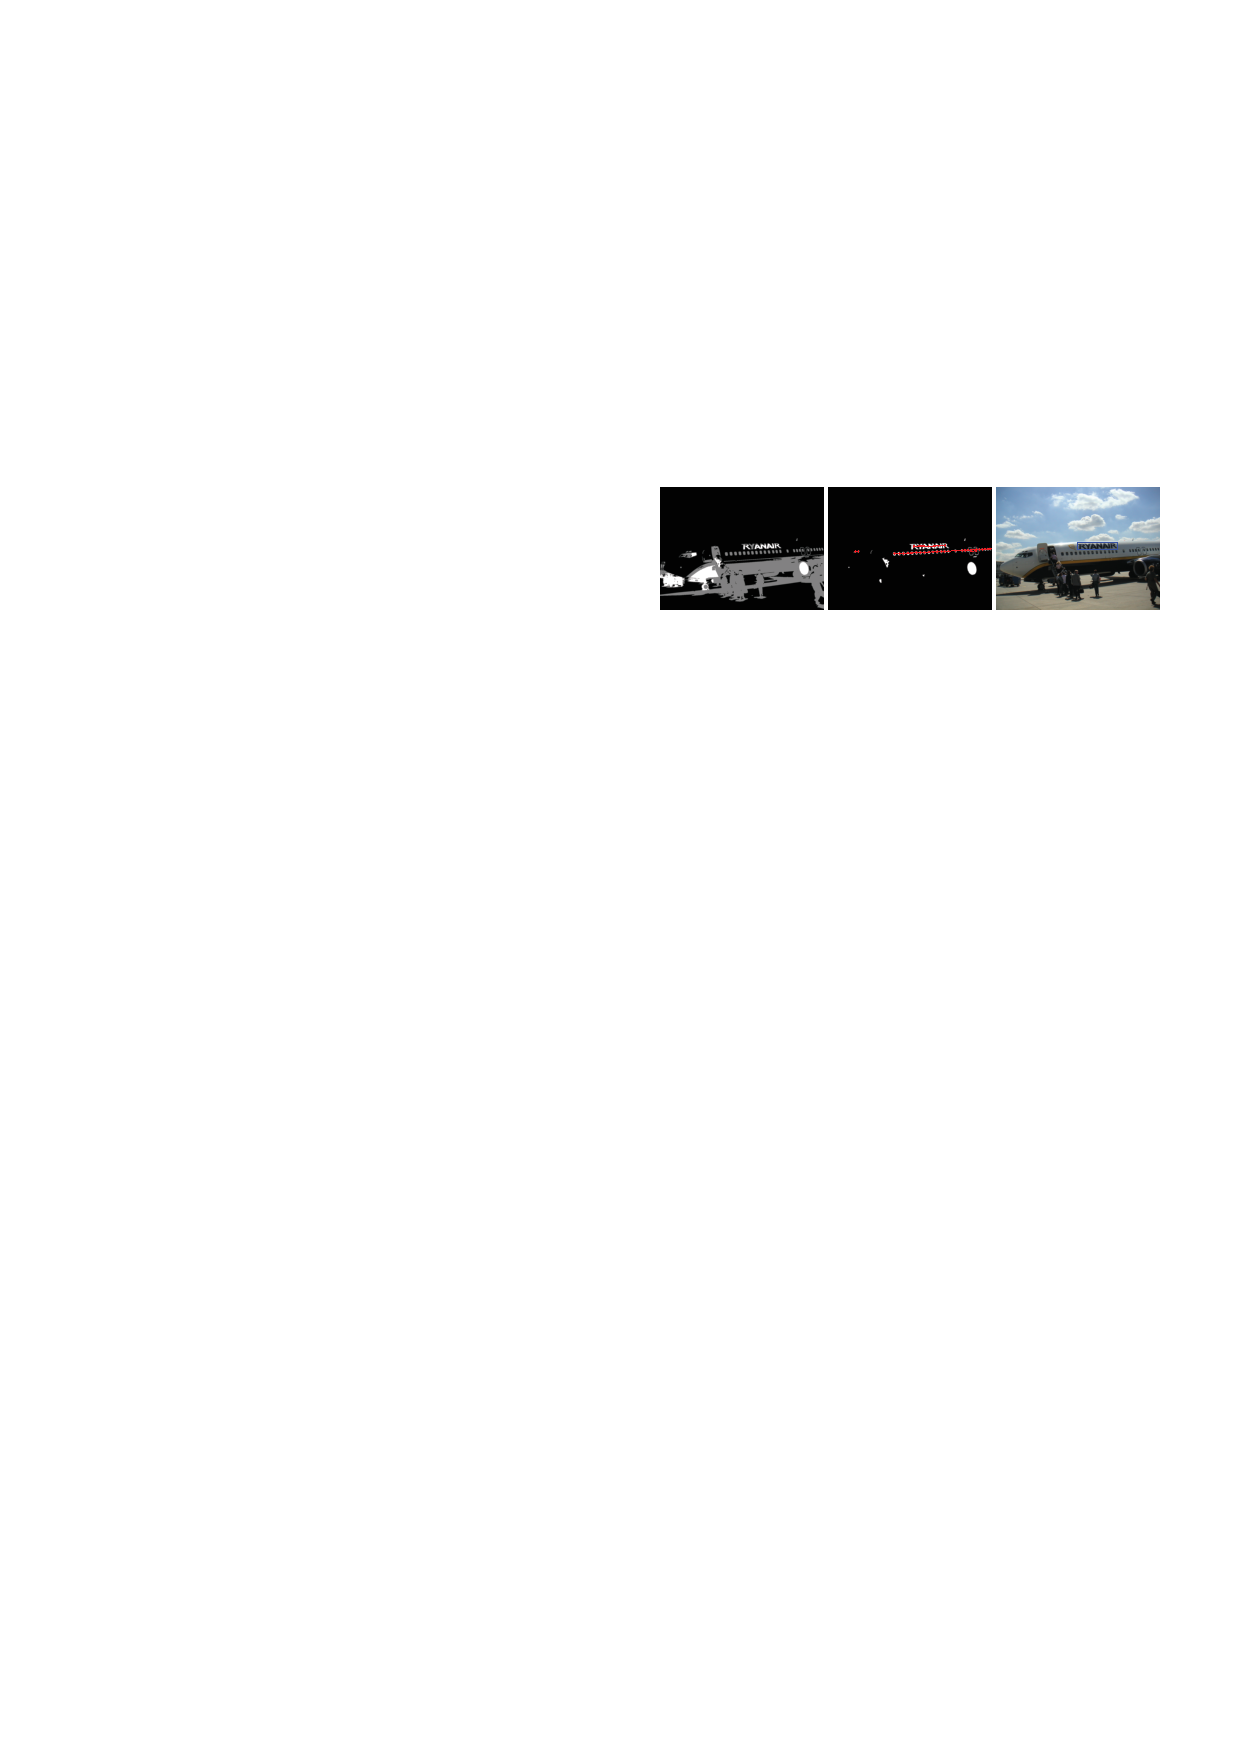
\includegraphics[width=\textwidth]{images/background/chen2011_mser}
  \caption[Using contrast-enhanced MSERs to detect text]{Extracting text from a natural image shown in \citet{Chen:2011ul}. \textit{From left to right:} Detected \glsplx{mser} of black-on-white objects; text candidates grouped to formed text lines after geometric and stroke width filtering; false positives rejected using text verification showing detected text in the blue box.}
  \label{fig:background:detection:cc:chen2011_mser}
\end{figure}

A significant requirement of all \gls{cc}-based techniques are the requirements to cluster extracted components back together again. This, in turn, also helps to remove any false positives by removing properties that don't meet set criteria. Various proposals have been made:

\begin{itemize}
  \item \citet{Epshtein:2010tj} use basic geometric filtering based on the stroke width detected and height ratios of candidates. Additionally, colours of candidates are averaged as it is expected that words be written in the same colour. These are then clustered into candidates pairs (of at least three letters), chained together if they share a similar direction.
  \item \citet{Zhang:2011cl} investigate the spacial relationship and property similarity of two neighbouring candidates, computing their link energies to compute \textit{text energy} (the probability a candidate is a true positive). The distance of the text energies are computed and, where beyond a set threshold, will be eliminated if not met. This is presented in \cref{fig:background:detection:cc:zhang2011_textenergy}.
  \item \citet{Zhang:2010wa} expand the use of graph spectrum, which has successfully been used in computer vision \citep{Sarkar:1996ig} to show image features in the form of a graph, use an adjacency matrix, then gather clusters of \glspl{cc} based on the positive eigenvectors of the graph. This process is illustrated in \cref{fig:background:detection:cc:zhang2010_graphspectrum}.
  \item \citet{Shivakumara:2011dn} propose the use of skeletal distance maps of a \gls{cc} to remove small artefacts and reduce false positives. They define \textit{simple} and \textit{complex} \glspl{cc} respectively as: (a) a single text string or false positive; (b) multiple text strings that are connected to each other. The skeletonisation process is shown in \cref{fig:background:detection:cc:shivakumara2010_skeleton}.
\end{itemize}
 
\begin{figure}[p!]
  \centering
  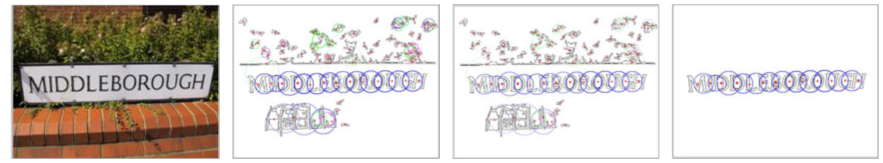
\includegraphics[width=\textwidth]{images/background/zhang2011_textenergy}
  \caption[Text energy for connecting candidates back together]{Using link and text energies for reconnecting character candidates shown in \citet{Zhang:2011cl}. \textit{From left to right:} original image; all link energies determined in a given image (note the false positives of background foliage); text energies calculated; all text energies greater than 0.5.}
  \label{fig:background:detection:cc:zhang2011_textenergy}
\end{figure}

\begin{figure}[p!]
  \centering
  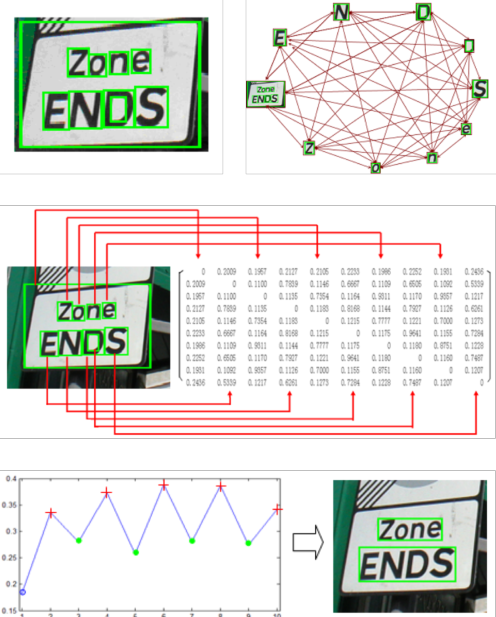
\includegraphics[width=0.5\textwidth]{images/background/zhang2010_graphspectrum}
  \caption[Using graph spectrum to cluster CCs]{Process of grouping components via graph spectrum \citep{Zhang:2010wa}. \textit{Top-left:} 10 \glspl{cc} detected. \textit{Top-right:} generated graph from detected candidates. \textit{Middle:} generated adjacency matrix. \textit{Bottom-left:} Positive eigenvector resulting from the graph spectrum. \textit{Bottom-right}: Resulting bounding boxes.}
  \label{fig:background:detection:cc:zhang2010_graphspectrum}
\end{figure}

\begin{figure}[p!]
  \centering
  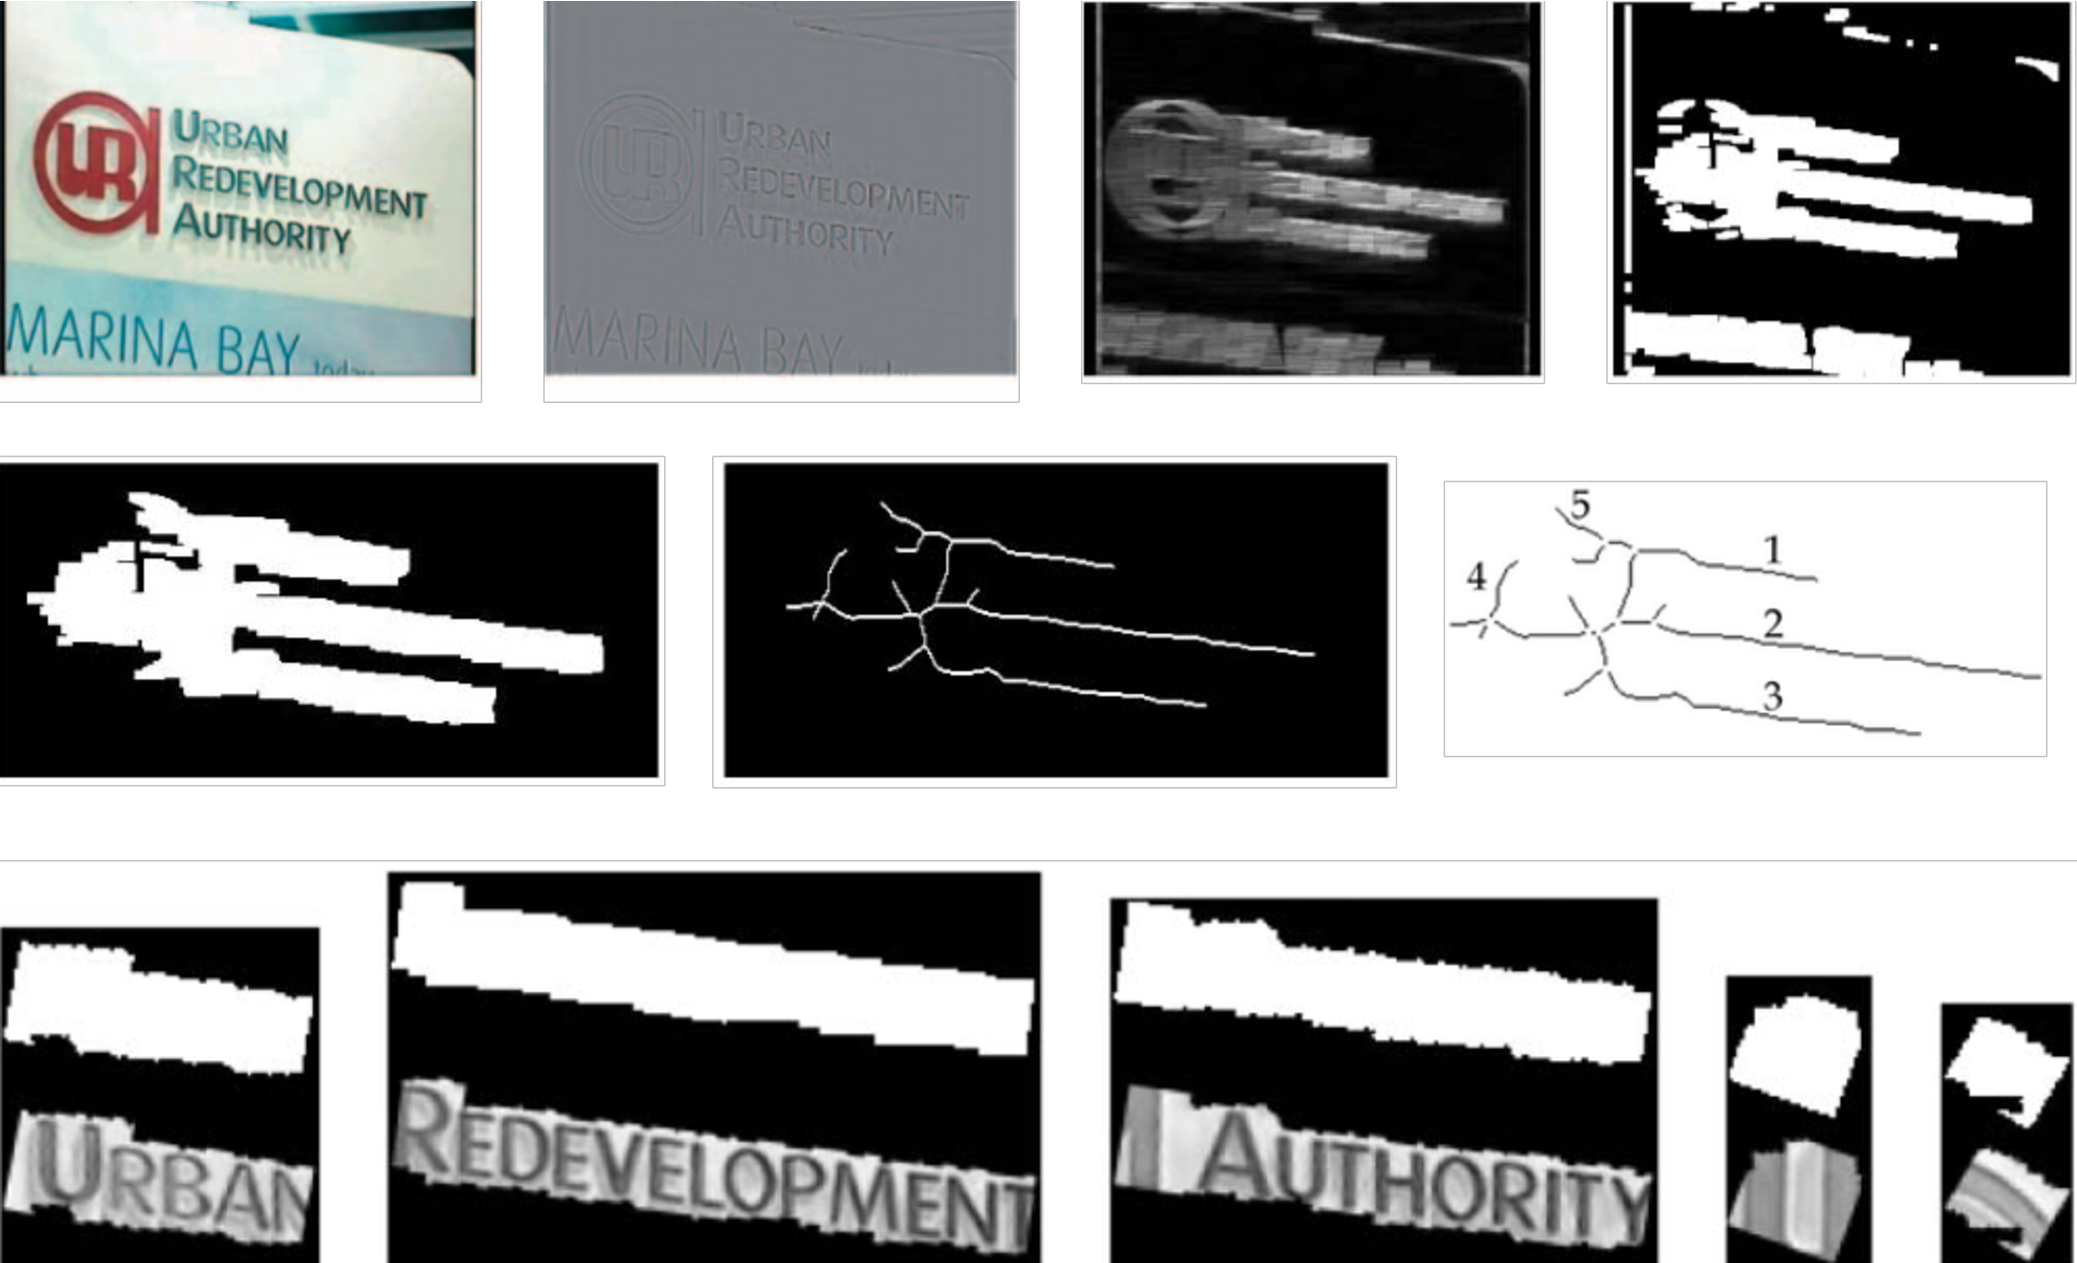
\includegraphics[width=\textwidth]{images/background/shivakumara2010_skeleton}
  \caption[Skeletonisation process of CCs]{Developing a skeletal map using the process proposed by \citep{Shivakumara:2011dn}. \textit{Top row:} Original image is processed using Fourier-Laplacian filtering. A maximum distance map is developed and parsed through a morphological operation to remove smaller artefacts. \textit{Middle row:} \gls{cc} classification and further skeletonisation, showing five labelled subcomponents. \textit{Bottom row:} The five sample subcomponents extracted from the skeletonisation process (in order). Note that subcomponents 4 and 5 are false positives.}
  \label{fig:background:detection:cc:shivakumara2010_skeleton}
\end{figure}

\clearpage

\subsection{Learning-based techniques}
\label{sec:detection:learning}

The learning-based approach has had a varied popularity over the years. While also referred to as a \textit{texture}-based approach, it typically utilises learning-based methods to train a classifier using these textures, considering text as a special texture within the image. This is done by extracting certain features over a portion of the image (i.e., the texture) either via heuristics or machine learning. The texture is typically extracted by scanning at varying scales, then classifying areas of pixels based on certain features. A classifier uses these features to identify text from non-text to extract text from its background.

Early works in the area focused primarily on how to classify a region as either text or non-text \citep{Sobottka:1999wi, Lienhart:2002ub, Li:2000uf, Kim:2003wj}. However, while it may be easy to procure training samples of text, it is often more difficult to procure non-text training samples \cite{Sung:1998vt,Heisele:2001ue} due to the wide variance of `non-text' samples, which need to be well-represented in the training set of the classifier.

A varied range of features have been utilised to mark textures. A recent feature made popular is the \gls{hog}, a object detection technique that utilises gradient orientation, first conceptualised in \citep{McConnell:1986wsb} and later coined by \citet{Freeman:1995uh}. However, its popularity did not become widespread until \citep{Dalal:2005jq}, where \citeauthor{Dalal:2005jq} showed its applicability was shown on pedestrian detection. Later, \gls{hog} was shown to be useful in text detection by \citet{Hanif:2008un}. Further features include: \gls{lbp} \citep{Ojala:1994hz}, which was shown to improve detection when combined with \gls{hog} \cite{Wang:2009wi}; wavelet energy \citep{Mohan:2001vb, Viola:2003ud}, which were applied to extract subtitles \citep{Gllavata:2004vq} and worked optimally with \gls{hog} in text extraction \citep{Pan:2010cj} (when compared to other features); Gabor filters \citep{Liu:2005et}; \gls{sift} descriptors \citep{Lowe:2004kp}; grey scale features \citep{Kim:2003wj}; \gls{surf} \cite{Bay:2008ud}, edge map features \cite{Chen:2004tj}; and shape contexts \citep{Belongie:2001uj}.

Many of these features can be combined and fed into a single or multiple classifiers \citep{Pan:2010cj, Hanif:2008un, Hanif:2009tm, Gllavata:2004vq, Ye:2005wu, Wang:2009il, Tu:2003tg}. Example classifiers include \glspl{svm} \citep{Cortes:1995wa,Burges:1998wd,Vapnik:1999vu}, the Adaptive Boosting (AdaBoost) classifier \citep{Freund:1996uc}---and variants thereof (\citep{Friedman:2000jg,Hanif:2009tm,Sochman:2005dn})---or \glspl{nn}, such as \glspl{mlp}, though \citet{Chen:2004tja} report that the use of \glspl{svm} showed better text texture verification than \glspl{mlp}. 

As shown in the wide range of features and classifiers, a main limitation of learning-based methods is the difficulty in selecting which combinations of features to use, the inability to detect sufficiently slanted text, as well as its reported high computational complexity due to the need to scan the image multiple time at different scales \citep{Li:2012wd, Epshtein:2010tj}. Furthermore, it is typical for these classifiers to required thousands of training images \cite{Chen:2004ux}.

More recently though, deep-learning \glspl{cnn} have been utilised for instance classification and per-pixel segmentation, as emphasised in \cref{fig:background:detection:learning:he2017_maskrcnn}. While \glspl{cnn} are a relatively old concept (see \citet{Lecun:1998hy}), they lost interest within image processing to \glsplx{svm} and AdaBoost throughout the late 1990s and 2000s. In \citeyear{Krizhevsky:2012wl}, however, \citet{Krizhevsky:2012wl} sparked interest in their use by demonstrating far increased classification accuracy within images in the ImageNet Large Scale Visualisation Recognition Challenge \citep{JiaDeng:2009dl}, with only a few modifications made to the \glspl{cnn} proposed by \citeauthor{Lecun:1998hy} more than a decade prior. 

This has since led to the rise of enhanced \glspl{cnn} such as FICS+++ \citep{Li:2016uj}, R-CNN \citep{Girshick:2014jx}, Fast/Faster R-CNN \citep{Girshick:2015vr, Ren:2017ug}, and Mask R-CNN \citep{He:2017ud}. A comparison of two of these networks using images in the Microsoft Common Objects in Context \cite{Lin:2014vm} dataset are shown in \cref{fig:background:detection:learning:he2017_maskrcnn}, with the Mask R-CNN framework illustrated in \cref{fig:background:detection:learning:he2017_maskrcnnframework}. The rise of these recent developments have sparked interest in multi-language machine learning libraries, such as MXNet\footnoteurl{http://mxnet.io}{30 June 2017}, which are able to combine these academic works for use in large-scale industry-focused production code \cite{Chen:2015vh}.

These methods are increasingly improving per-pixel classification of objects within natural scenes. However, applicability of these deep-learning networks in the sole context of \textit{text extraction} is yet to be widely explored, though a \citeyear{Jaderberg:2016wj} paper by \citet{Jaderberg:2016wj} did show the viability of a real-time text reading pipeline based on \glspl{cnn} (\cref{fig:background:detection:learning:jaderberg2016_cnn}) that successfully extracts any text query from 2.3 million frames of BBC News footage\footnoteurl{http://zeus.robots.ox.ac.uk/textsearch}{14 August 2017}.

\begin{figure}[h]
  \centering 
  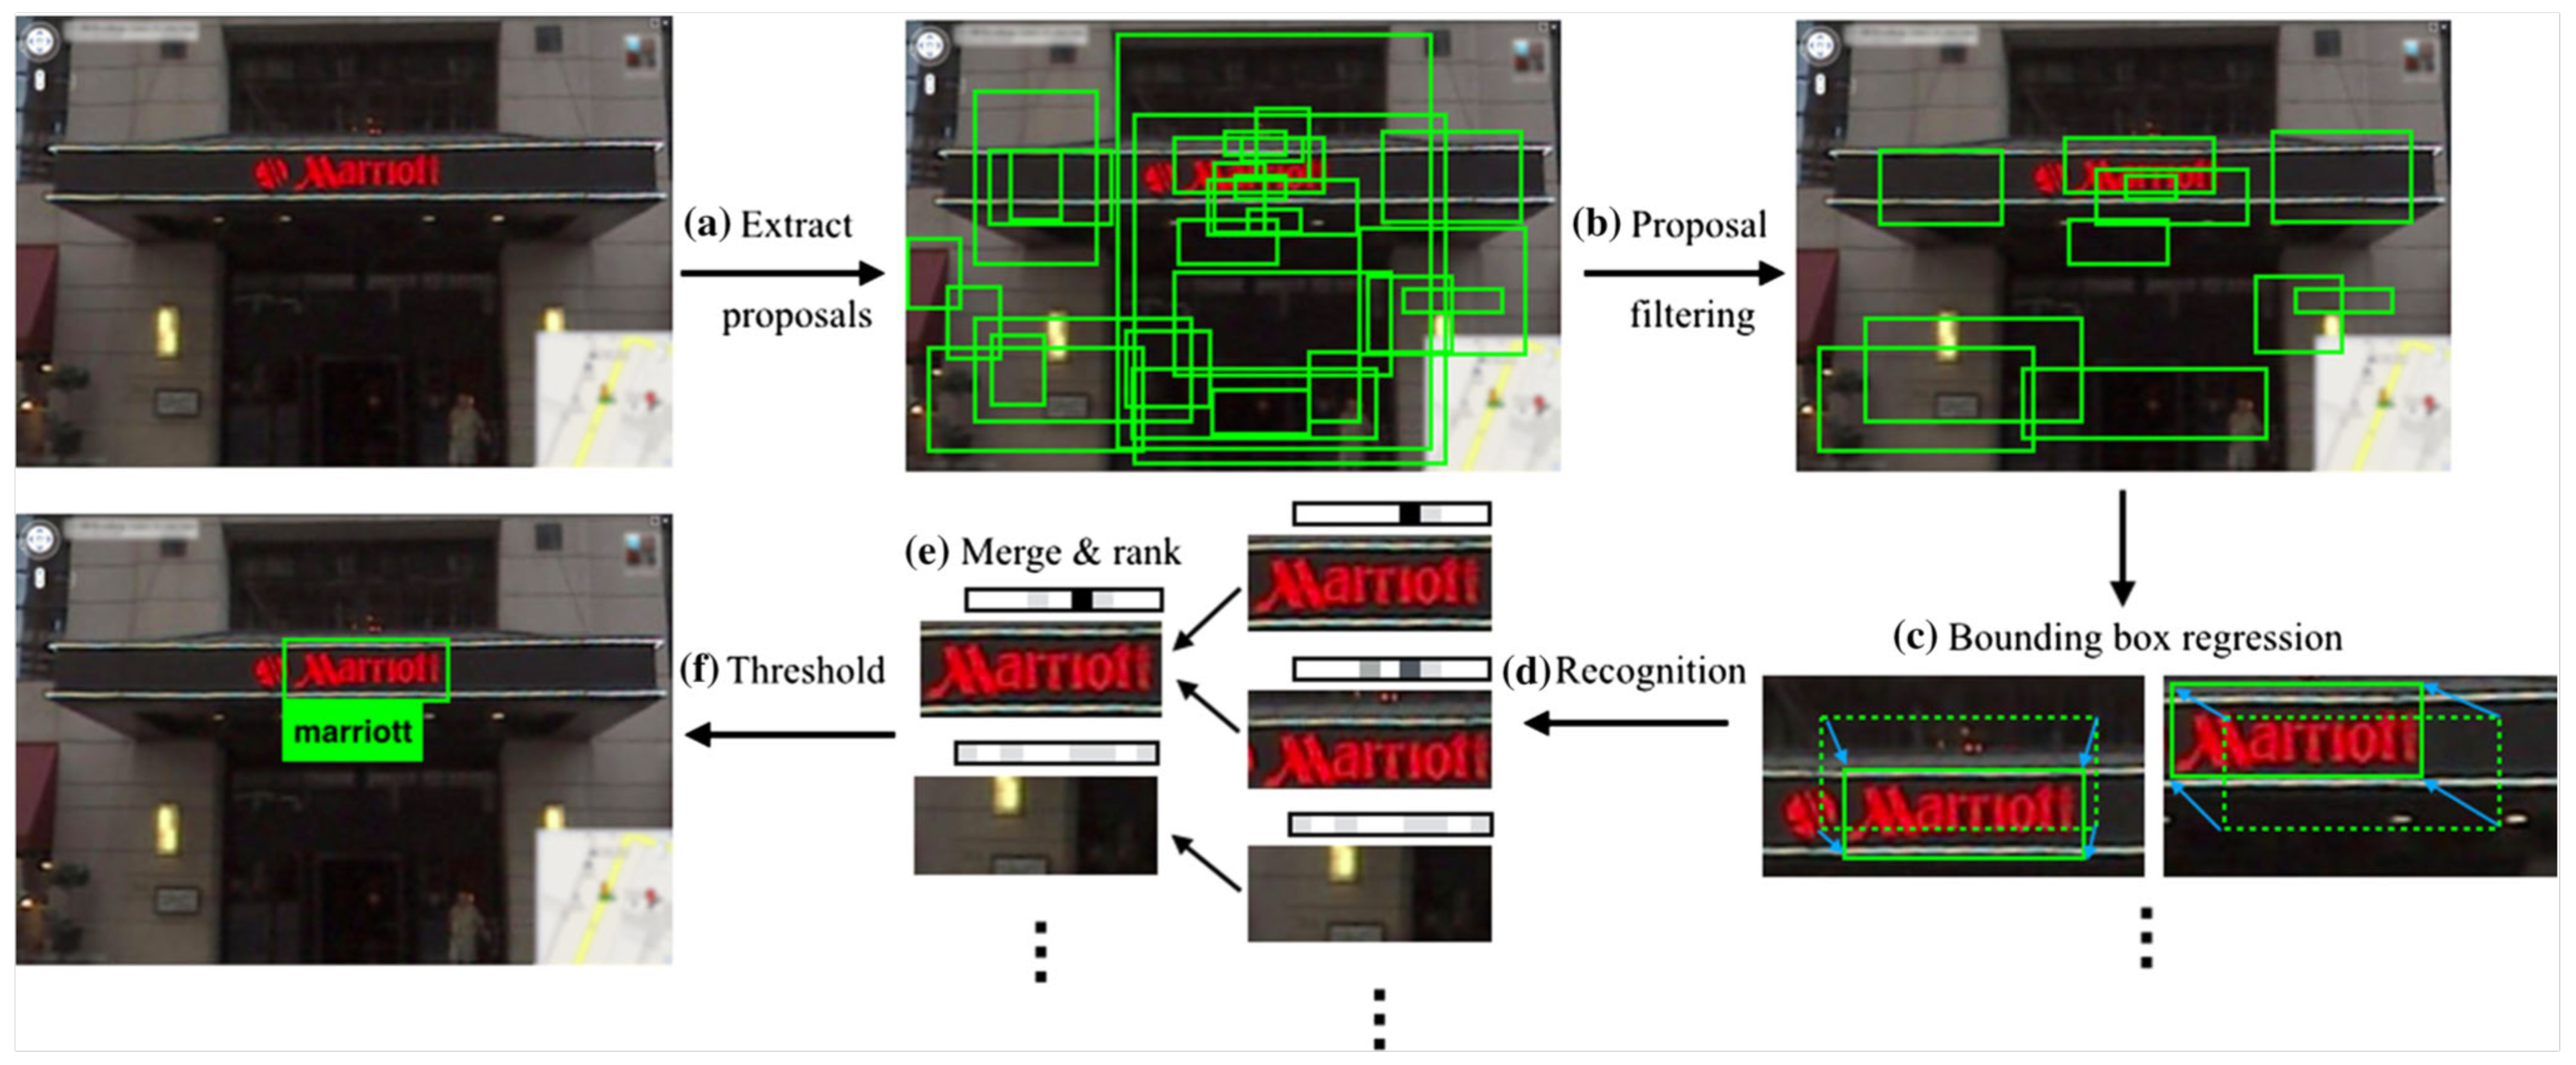
\includegraphics[width=\textwidth]{images/background/jaderberg2016_cnn}
  \caption[A pipeline for text extraction using CNNs]{The pipeline for text extraction proposed in \citep{Jaderberg:2016wj}.}
  \label{fig:background:detection:learning:jaderberg2016_cnn}
\end{figure}

\begin{figure}[p]
  \centering
  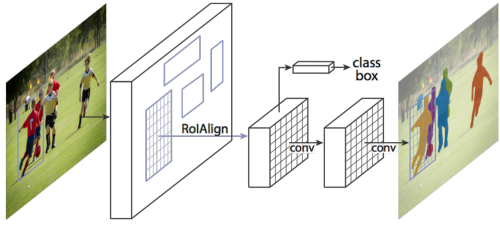
\includegraphics[width=\textwidth]{images/background/he2017_maskrcnnframework}
  \caption[The Mask R-CNN framework for instance segmentation]{The Mask R-CNN framework for instance segmentation \citep{He:2017ud}.}
  \label{fig:background:detection:learning:he2017_maskrcnnframework}
\end{figure}

\begin{figure}[p]
  \centering
  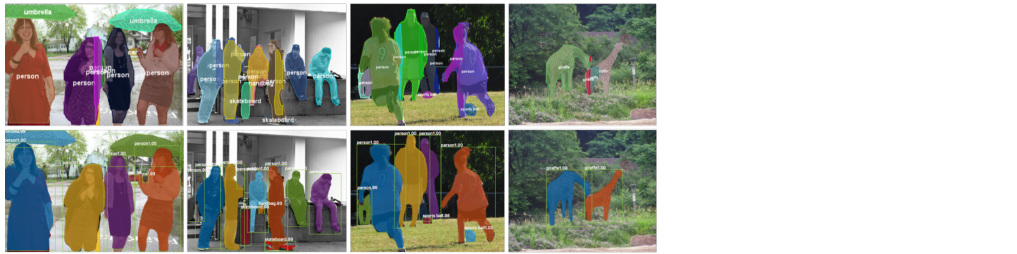
\includegraphics[width=\textwidth]{images/background/he2017_maskrcnn}
  \caption[Use of CNNs for object detection]{Use of \glspl{cnn} have recently been shown to have accurate per-pixel object detection and classification. \textit{Top row:} FCIS+++ \citep{Li:2016uj}. \textit{Bottom row:} Mask R-CNN \citep{He:2017ud}. Mask R-CNN outperforms FICIS+++ for overlapping instance segmentation.}
  \label{fig:background:detection:learning:he2017_maskrcnn}
\end{figure}

\clearpage